\documentclass[a4paper,11pt]{article}

\usepackage[utf8]{inputenc}

\usepackage{graphicx}
\usepackage{caption}
\usepackage{subcaption}

\usepackage{pgfplots}
\usepackage{float}
\usepackage{hyperref}
\usepackage{soul}
\hypersetup{
    colorlinks=true, % Enable colored links
    linkcolor=black, % Color for internal links
    urlcolor=black,  % Color for external links
    citecolor=black, % Color for citation links
    pdfborder={0 0 0}, % Remove border around links
}
\newcommand{\underlinehref}[2]{%
    \href{#1}{\ul{#2}}%
}
\pgfplotsset{compat=1.18}


\usepackage{minted}

\begin{document}

    \title{
        \textbf{Trees in C}
    }
    \author{Péter Herczku}
    \date{Fall 2024}

    \maketitle

    \section*{Introduction}

    The task is to implement the tree data structure along with its operations.
    We also needed to investigate the depth first traversal method for printing the tree in order.

    I completed the assignment using the C programming language.

    \section*{Trees}

    A tree is similar to a linked list, but a node can link to more than one node.
    In this assignment we looked at binary trees which means that each node has at most two branches.
    The reason we call this a tree is because we have a top node which is the root and all other branches come from that same element.
    
    Sorted binary trees require their elements to be comparable. 
    In the assignment I used integers because they satisfy this condition and are easy to work with.

    \subsection*{Methods}

    \begin{itemize}
        \item \textbf{add(tree* tr, int item)} - adds an element to the tree while keeping it sorted
        \item \textbf{lookup(tree* tr, int item)} - looks up a node which the value {\tt item}
     \end{itemize}

     We also need methods that create a tree and destroy them. 
     Let's take a look at our implementation now.
     For the add method we can choose to implement it recursively or not. First, we investigate the recursive approach:

     \begin{minted}{c}
void add_node(node* nd, int value) {
    if (nd->value == value) return;
    if (value < nd->value) {
        if (nd->left == NULL) {
            nd->left = construct_node(value);
        } else {
            add_node(nd->left, value);
        }
    } else {
        if (nd->right == NULL) {
            nd->right = construct_node(value);
        } else {
            add_node(nd->right, value);
        }
    }
}
     \end{minted}

     This algorithm finds the appropriate spot for the new node, while keeping the tree sorted.
     Since the branches of a tree are still trees we can do it recursively, but C cannot recognize that our branches are subtrees, therefore we need to create another method that takes a tree as an argument:

     \begin{minted}{c}
void add_recursive(tree *tr, int value) {
    if(tr->root == NULL) tr->root = construct_node(value);
    else add_node(tr->root, value);
}
     \end{minted}

    We can also implement this method without recursion.
    The implementation is almost the same as before but we need to keep track of where we are in the tree, by having a current variable.
    \begin{minted}{c}
void add(tree *tr, int value) {
    if(tr->root == NULL) {
        tr->root = construct_node(value);
        return;
    }
    node *curr = tr->root;
    while(1) {
        if(curr->value == value) break;
        if(value < curr->value) {
            if (curr->left == NULL) {
                curr->left = construct_node(value);
                break;
            }

            curr = curr->left;
        }
        if(value > curr->value) {
            if (curr->right == NULL) {
                curr->right = construct_node(value);
                break;
            }

            curr = curr->right;
        }
    }
}
    \end{minted}


     Now we can look at the lookup function, which is quite similar to implement: we recursively traverse the tree until we find the value we are looking for.
     Let's take a look at our implementation:
     \begin{minted}{c}
bool lookup(tree *tr, int value) {
    if(tr->root == NULL) return false;
    node *curr = tr->root;
    while(1) {
        if (curr->value == value) return true;
        if (value < curr->value && curr->left != NULL) {
            curr = curr->left;
        } else if(value > curr->value && curr->right != NULL) {
            curr = curr->right;
        } else {
            return false;
        }
    }
}
    \end{minted}

    In theory, if we have a balanced tree - so that the two branches from root has the same depth - this algorithm should have a time complexity of $O(log(n))$.
    The worst case occurs when our tree looks like a linked list, in this case the time complexity becomes $O(n)$.
    Let's benchmark and compare our results to the theoretical assumptions:

    \begin{figure}[H]
        \centering
        \begin{subfigure}[b]{.5\textwidth}
            \centering
            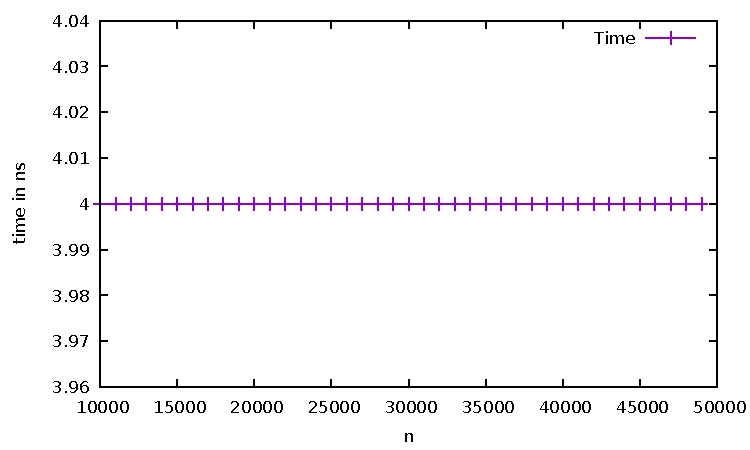
\includegraphics[width=\textwidth]{./src/data} % Adjust width or height as needed
        \end{subfigure}
        \caption{Graph of lookup}
        \label{fig:graph_1}
    \end{figure}

    The graph shows linear relationship, which is due to the fact that we are adding the elements after each other from 1 to n, therefore our tree looks like a linked list.
    
    The idea behind this method is quite similar to binary search where we basically did the same thing.
    However, as previously mentioned, the tree is not always balanced therefore this algorithm has worse time complexity compared to binary search.

    \section*{Depth first traversal}

    Throughout the report, we used a sorted tree where the smaller values are to the left, and the larger ones are to the right.
    Therefore, if we want to go through the tree in order, we should start looking up the leftmost value first.
    This approach is called depth first traversal, because we are going down as deep as we can first, in order to traverse the tree.
    Let's look at our implementation:
    \begin{minted}{c}
void print(node *nd) {
    if (nd != NULL) {
        print(nd->left);
        printf("%d ", nd->value);
        print(nd->right);
    }
}

void print_tree(tree *tr) {
      if (tr->root != NULL)
        print(tr->root);
      printf("\n");
}
    \end{minted}

    We can also do this without recursion, by using a stack.
    First, we go down as deep as we can while pushing our nodes onto the stack.
    After reaching the leftmost node, we pop the stack and print out the result.
    Then we check, if it has any elements to the right:
    if it does, we go there and do the following, but if not, we pop the stack again and print out the next value.
    \begin{minted}{c}
stack *stk = new_stack();
node *cur = tr->root;
    
while(cur->left != NULL ) {
    push(stk, cur);
    cur = cur->left;
}

while(cur != NULL) {
    printf("%d ", cur->value);

    if(cur->right != NULL) {
        cur = cur->right;
        while(cur->left != NULL) {
            push(stk, cur);
            cur = cur->left;
        }
    } else {
        cur = pop(stk);
    }
}
    \end{minted}


    \section*{GitHub}
    I have uploaded the full project to \underlinehref{https://github.com/peterherczku/ID1021/tree/main/assignment-7}{my github repository}, where we can find the code used to make this report.

\end{document}
